%Resume penggunaan aplikasi testis webservice
%judul jurnal IMPLEMENTASI REST WEB SERVICE UNTUK SALES ORDER DAN SALES TRACKING BERBASIS MOBILE
%Kelompok 5 D4 TI - 2B
%Fransiscus Ivan Martongam      1164039
%Lalita Chandiany Adiputri      1164043
%Eko Cahyono Putro              1164035
%Lidwina Triniska Gulo          1164044
%Sulpadianti Bunyamin           1164096


\section{Pengenalan WebService}
Web Services dengan arsitektur REST digunakan oleh berbagai macam jenis client seperti mobile, Web, dan Desktop.
Dapat membantu perusahaan untuk melakukan pelacakan, tracking terhadap tenaga penjual yang ditugaskan untuk menawarkan 
barang atau penagihan ke pelanggan. Dengan REST Web Services yang akan dibuat perusahaan akan dapat memastikan
bahwa semua tenaga penjual akan mengunjungi pelanggan sesuai dengan target yang sudah ditentukan oleh perusahaan.


\section{Arsitektur Web Services}
Architektur Web Service memiliki tiga komponen utama diantaranya yaitu Service provider adalah Penyedia web service yang berfungsi
menyediakan kumpulan web services yang dapat diaksesoleh pengguna.Service requesto adalah aplikasi yang bertindak sebagai pengguna yang
melakukan permintaan layanan (berupaweb services) keservice provider.Service registry adalah tempat dimana service provider 
mempublikasikan layanannya. Pada arsitekturWeb service,Service registry bersifat opsional.

\ref{arsitektur}
\centerline{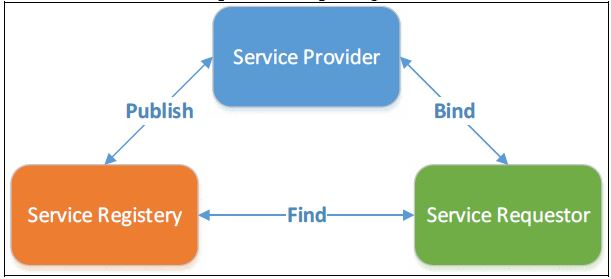
\includegraphics[width=1\textwidth]{figures/arsitektur.PNG}}
\caption{arsitektur web service}
\lable{arsitektur}
\end{figure}


\section{rest dalam penggunaan testing web service}
REST adalah filosofi desain yang mendorong untuk menggunakan protokol dan fitur yang sudah ada pada Web. Pada web services akan dapat memaksimalkan kinerja web services terutama pada performa, skalabilitas, dan kemudahan untuk dimodifikasi. Bentuk web service menggunakan REST style digunakan sebagai backend dari aplikasi berbasis mobile karena cara aksesnya  mudah dan hasil data yang dikirimkan berformat JSON sehingga ukuran file menjadi lebih kecil. 
